\section{Действия и награды} \label{ch2:act-rew} %название по-русски

\subsection{Архитектура ветвления действий (Action Branching)}

Обычно довольно трудно исследовать проблемы с многомерными пространствами действий. Архитектура \textit{ветвления действий} предназначена для решения таких проблем. Например, в среде с \textit{N}-мерным пространством действий и $d_n$ дискретных последующих действий для каждого измерения \textit{n} необходимо рассмотреть в общей сложности $\Pi^N_{n=1} d_n$ возможных действий \cite{tavakoli2017action}. Правильно спроектированные разветвлённые архитектуры действий могут эффективно и результативно исследовать такое большое многомерное пространство действий \cite{tavakoli2017action}.

\begin{figure}[ht!]
    \center
    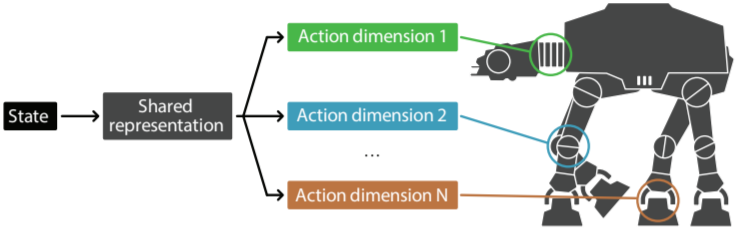
\includegraphics [scale=0.4] {my_folder/images/ch2/action-branching.png}
    \caption{Архитектура сети для ветвления действий, например, для робота, где сеть принимает состояние в качестве входных данных и разделяет нижние уровни для извлечения представлений признаков, а затем расходится по ветвям для относительно независимых под-действий, включая, например, высказывание, действие рукой, действие ногой и т.д. Основано на \cite{tavakoli2017action}}
    \label{fig:ch2-action-branching}
\end{figure}

Основной идеей архитектуры является модуль совместного принятия решений, который извлекает скрытое представление из входного наблюдения и создаёт отдельные выходные ветви для каждого измерения действия. На рисунке \firef{fig:ch2-action-branching} представлена архитектура \textit{ветвления действий}. \textit{n} измерений действий представляют собой \textit{n} относительно независимых под-действий.

В архитектурах \textit{ветвления действий} значения \textit{Q} рассчитываются для каждого измерения действия. Тем не менее, мы бы хотели, чтобы многомерное действие оценивало одно единственное \textit{Q}-значение, выводимое сетью критика.

\subsection{Архитектура гибридного вознаграждения}

Как показано в \cite{seijen2017hybrid}, жизненно важно иметь точную оптимальную value-функцию в обучении с подкреплением, поскольку она оценивает ожидаемую награду как сигнал для оптимизации политики. Как только оптимальная value-функция изучена, из неё можно получить оптимальную политику.

\begin{figure}[ht!]
    \center
    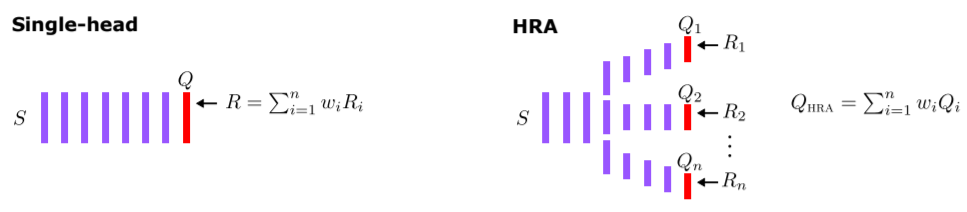
\includegraphics [scale=0.80] {my_folder/images/ch2/hybrid-reward.png}
    \caption{Глубокая нейронная сеть с одной головой, аппроксимирует одну единственную Q-функцию с глобальной функцией награды (слева), и Q-сеть с гибридной архитектурой вознаграждения (справа). Сеть имеет n голов, аппроксимирующих n Q-функций. Каждая Q-функция оценивает Q-значение с помощью соответствующей разложенной функции награды. Основано на \cite{seijen2017hybrid}}
    \label{fig:ch2-hybrid-reward}
\end{figure}

Более того, две разные value-функции могут привести к одной и той же политике, когда агент действует жадно в соответствии с ними \cite{seijen2017hybrid}. Следовательно, можно было бы изучить несколько более простых value-функций, если изучить сложную value-функцию сложно или даже невозможно. В таком случае глобальная функция награды может быть соответственно разложена на несколько различных функций награды:

\begin{equation}
    \begin{multlined}
        R_{rev}(s, a, s') = \sum^n_{k=1} R_k (s, a, s')
    \end{multlined}
\end{equation}

где $R_{rev}$ - глобальная функция награды, которая разбита на \textit{n} функций награды. Каждая разложенная функция награды зависит от подмножества состояний и имеет свою собственную функцию \textit{Q}-значения. Глубокая \textit{Q}-сеть с общими нижними слоями и \textit{n} головами используется для аппроксимации \textit{n} \textit{Q}-значений, обусловливающих текущее состояние и действие с различными функциями разложения награды \firef{fig:ch2-hybrid-reward}.

\begin{equation}
    \begin{multlined}
        Q_{H R A}(s, a; \theta) := \sum^n_{k=1} Q_k(s, a;\theta)
    \end{multlined}
\end{equation}

Q-сеть затем итеративно улучшается за счёт оптимизации функции потерь

\begin{equation}
    \begin{multlined}
        L_i(\theta_i) = \mathbb{E}_{s, a, r, s'}[\sum^n_{k=1}(y_{k, i}-Q_k(s, a;\theta_i))^2]
    \end{multlined}
\end{equation}

где

\begin{equation}
    \begin{multlined}
        y_{k, i} = R_k(s, a, s') + \gamma \max_{a'} Q_k(s', a';\theta_{i-1})
    \end{multlined}
\end{equation}

$\theta_i$ — это веса Q-сети в текущей итерации \textit{i}, а $\theta_{i-1}$ - веса отдельной целевой сети в предыдущей итерации.
В гибридной архитектуре вознаграждений \textit{n} \textit{Q}-значений выводятся \textit{n} головами из одной единственной \textit{Q}-сети. Однако для того, чтобы иметь консистентный градиент для улучшения политики для каждого измерения действий, следует создавать отдельные \textit{Q}-сети для оценки \textit{Q}-значений для каждого измерения действий.
